\documentclass[12pt, a4paper]{article}

% Packages
\usepackage[utf8]{inputenc}
\usepackage{geometry}
\geometry{top=2.5cm, bottom=2.5cm, left=2.5cm, right=2.5cm}
\usepackage{graphicx}
\usepackage{tabularx}
\usepackage{hyperref}
\usepackage{float}
\usepackage{titlesec}
\usepackage{booktabs}
\usepackage{amsmath}
\usepackage{indentfirst}
\usepackage{tocloft}
\usepackage{tikz}
\usetikzlibrary{positioning,arrows.meta,shapes.geometric}

% Section formatting to match the Word document style
\titleformat{\section}{\normalfont\Large\bfseries}{\thesection.}{1em}{}
\titleformat{\subsection}{\normalfont\large\bfseries}{\thesubsection.}{1em}{}

\begin{document}

% -------------------------------------------------------------------
% TITLE PAGE
% -------------------------------------------------------------------
\begin{titlepage}
    \begin{center}
        % Header with placeholders for WUT and Faculty logos
% Header Image
        
\includegraphics[width=\textwidth]{proj/header.png} \\[1cm]
        
        \vspace{2cm}
        % Adjusted spacing to account for the image
        % \begin{tabular}{c}
        %     \textbf{\Large WARSAW UNIVERSITY OF TECHNOLOGY} \\[0.2cm]
        %     \textbf{\Large Faculty of Mathematics} \\[0.2cm]
        %     \textbf{\Large and Information Science}
        % \end{tabular}        
        % \vspace{3cm}
        
        \textbf{\LARGE Artificial Intelligence Fundamentals} \\[1cm]
        \textbf{\Huge Exoplanet Visualization Agent} \\[2cm]
        
        \textbf{\Large Authors:} \\[0.5cm]
        \Large Aleksander Jeżowski \\
        \Large Denis Lisovytskiy \\
        \Large Piotr Czechowski \\
        \Large Rafał Lasota \\[2cm]
        
        \textbf{\Large Computer Science and Information Systems} \\[1cm]
        \textbf{\Large 01.04.2026}
    \end{center}
\end{titlepage}

\newpage


\section*{Responsibilities}
\begin{table}[H]
    \centering
    \begin{tabularx}{\textwidth}{l X}
        \toprule
        \textbf{Name} & \textbf{Tasks} \\
        \midrule
        Aleksander Jeżowski & Report - Description of a problem, Astrophysics Engine, Simulation results, GUI implementation (Streamlit) \\
        Denis Lisovytskiy & Report - Analysis of a problem, AI implementation (PINNFormer), AI implementation (ELM \& CTGAN), RAG Citations, Web deployment \\
        Piotr Czechowski & Report - Existing Solutions, The description of the preferred solution, GUI implementation (Streamlit) \\
        Rafał Lasota & Report - Conclusions, LLM Agent setup, AI implementation (ELM \& CTGAN), RAG Citations, Web deployment \\
        \bottomrule
    \end{tabularx}
\end{table}
\newpage


% -------------------------------------------------------------------
% TABLE OF CONTENTS
% -------------------------------------------------------------------
\tableofcontents
\newpage

% -------------------------------------------------------------------
% 1. DESCRIPTION OF A PROBLEM
% -------------------------------------------------------------------
\section{Description of a problem}

Our project focuses on creating an Autonomous Exoplanetary Digital Twin to quickly evaluate the climate and habitability of exoplanets. 

To prepare the final solution, we must address the fundamental challenge in astrobiology: determining which of the 5,700+ confirmed exoplanets can support life. Reconstructing a planet's climate profile-including surface temperature distribution and habitability zones-requires complex calculations. 

In the first part, the main goal is to evaluate habitability using General Circulation Models (GCMs). However, running a standard 3D GCM (like NASA's ROCKE-3D) for a single planetary configuration takes 2 to 7 days on a supercomputer. This computational cost makes it impossible to systematically scan thousands of discovered exoplanets.

The penultimate step is to bypass these heavy computations by using AI algorithms and Machine Learning to act as physics-informed surrogate models. We need a system that can take raw exoplanet data (stellar host temperature, radius, orbital distance, etc.) and generate 3D surface temperature maps and scientific habitability metrics in seconds rather than days, while answering critical questions like "What is the climate state (Eyeball, Lobster, or Greenhouse)?" and "What is the false-positive risk for biosignatures?"


\begin{figure}[htbp]
    \centering
    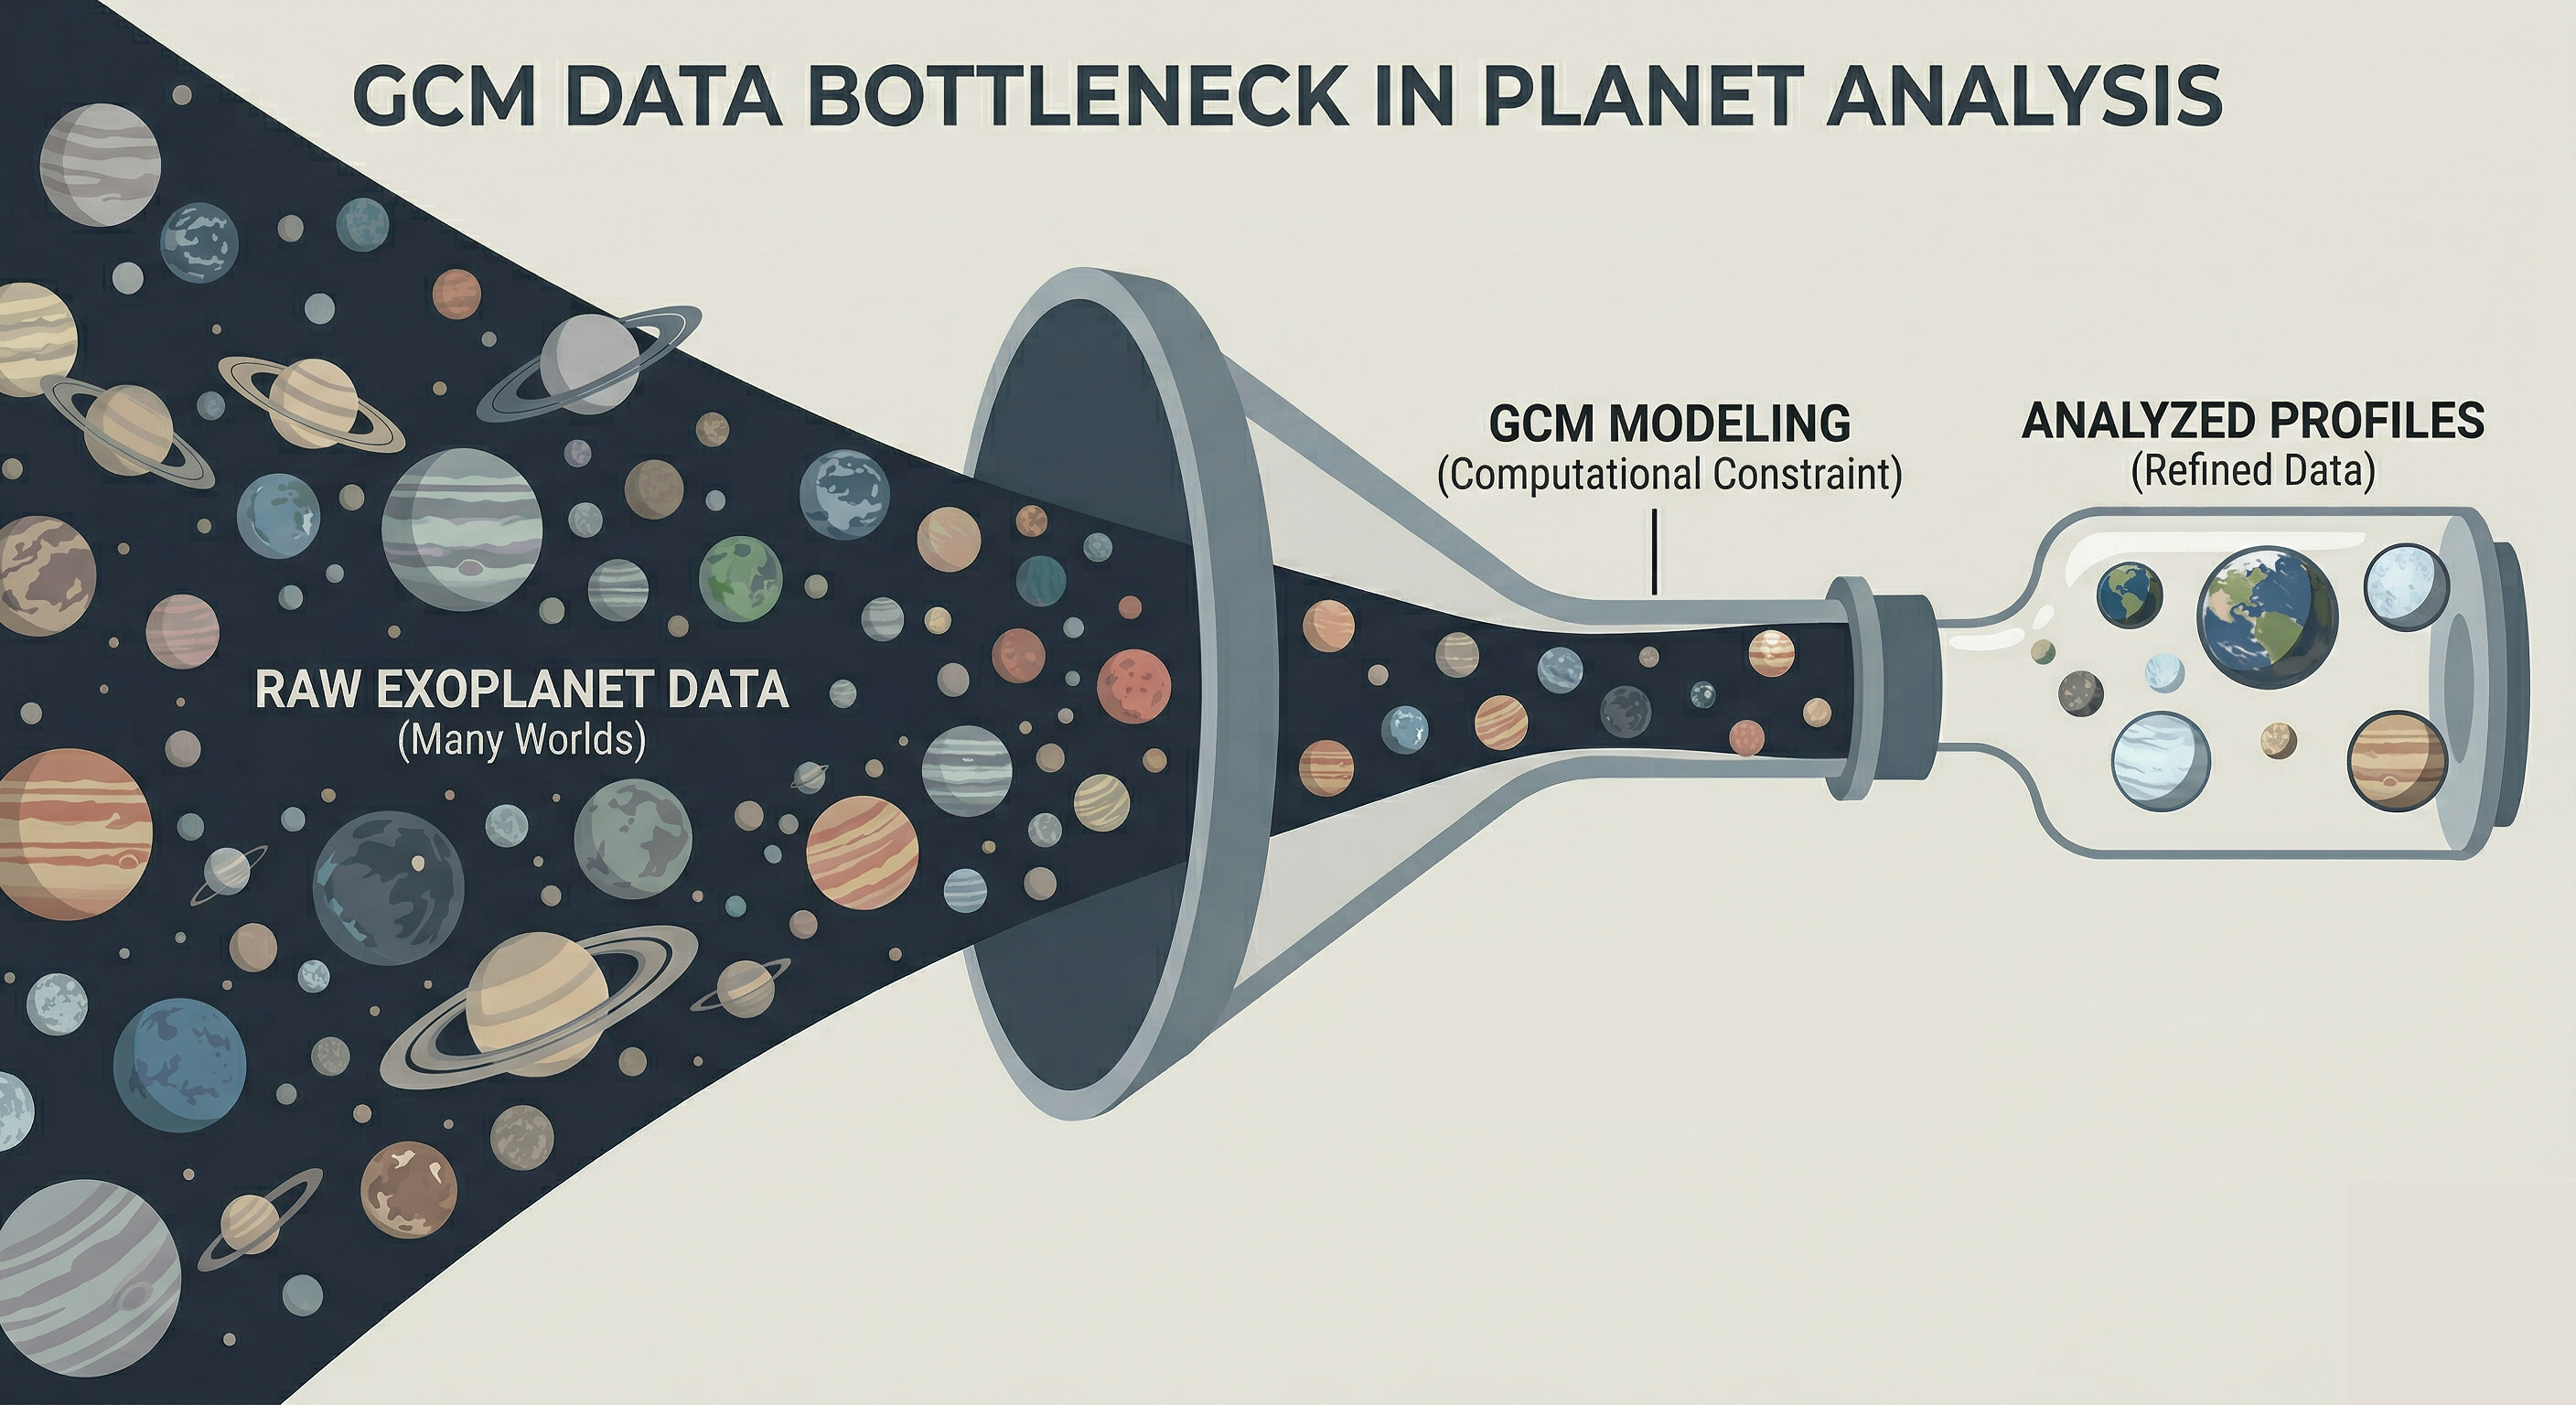
\includegraphics[width=0.9\textwidth]{proj/diag.png}
    \caption{Visualizing the data transition to our Exoplanet Visualization Agent.}
    \label{fig:proj-desc}
\end{figure}
\newpage

% -------------------------------------------------------------------
% 2. AN ANALYSIS OF A PROBLEM
% -------------------------------------------------------------------
\section{An analysis of a problem}

The first step is addressing the extreme class imbalance in planetary data.
In the NASA Exoplanet Archive, there are roughly 5,700 confirmed planets, but only about 60 are considered potentially habitable (having an Earth Similarity Index $>$ 0.8). This extreme imbalance ($\approx 1:380$ ratio) causes standard ML models to suffer from statistical collapse, where they simply learn to predict the majority class and fail to reproduce complex climate topologies like the "eyeball" state.

Another major issue is physical hallucinations. Using Large Language Models (LLMs) to interpret or generate scientific claims often leads to non-physical results (e.g., negative Kelvin temperatures or impossible mass-radius ratios). Therefore, the system requires strict programmatic guardrails (validators) to ensure thermodynamic constraints and energy conservation are preserved.

\newpage


% -------------------------------------------------------------------
% 3. EXISTING SOLUTIONS
% -------------------------------------------------------------------
\section{Existing solutions}

There are existing solutions for modeling exoplanetary climates and habitability, divided mainly into two extremes.

For example, high-fidelity 3D General Circulation Models (GCMs) like NASA ROCKE-3D and the LMD Generic GCM. These models solve Navier-Stokes equations for atmospheric flow over a 3D grid with a time-step of ~30 minutes until equilibrium is reached (simulating $\sim 10^4$ years). While highly accurate, they require HPC clusters and days of computation per planet.

On the other hand, we have 1D analytical models and simple statistical indices like the Earth Similarity Index (ESI) or the Surface Exoplanetary Planetary Habitability Index (SEPHI). These are very fast to compute but lack the spatial depth required to analyze localized climate states, such as terminator zone habitability on tidally locked planets.

\newpage



% -------------------------------------------------------------------
% 4. THE DESCRIPTION OF THE PREFERRED SOLUTION
% -------------------------------------------------------------------
\section{The description of the preferred solution}

\textbf{Programming Language:} Python 3.10+ \\
\textbf{The most important libraries:} Streamlit (GUI), scikit-elm, PyTorch, CTGAN, LangChain, Ollama, Plotly. \\

For our digital-twin-inspired surrogate, we use a multi-layered architecture combining generative AI, fast ML surrogates, and strict physical guardrails. 

Our application is built using Streamlit, providing an interactive 5-tab web interface. Users can query real observational data from the NASA Exoplanet Archive using Table Access Protocol (TAP/ADQL). In addition, our catalog-building pipeline merges multiple public data sources (NASA, Exoplanet.eu, DACE, and Gaia) into a normalized table used for analysis and training workflows. The core calculation engine computes physics-based habitability indices, such as equilibrium temperature ($T_{eq}$), ESI, SEPHI scores, and Kopparapu (2013) Habitable Zone boundaries.

To handle AI orchestration, we use a dual-LLM setup via LangChain and local Ollama inference. The system uses Qwen 2.5-14B as an orchestrator for tool calling, and AstroSage-Llama-3.1-8B as a domain expert to interpret the raw numerical outputs into scientific narratives. We also support runtime modes for different hardware profiles: Dual-LLM mode, Single-LLM mode, and Deterministic mode (without LLM narrative generation). Crucially, all data passes through Pydantic validators to reject unphysical inputs or outputs (e.g., preventing inputs exceeding the deuterium-burning limit of $\sim 13$ Jupiter masses).

To improve reliability, we implemented a graceful degradation and fallback chain. If higher-level components are unavailable (e.g., LLM runtime or selected surrogate), the application degrades to deterministic physics tools and simpler climate approximations while preserving result availability and UI continuity.

\begin{figure}[H]
    \centering
    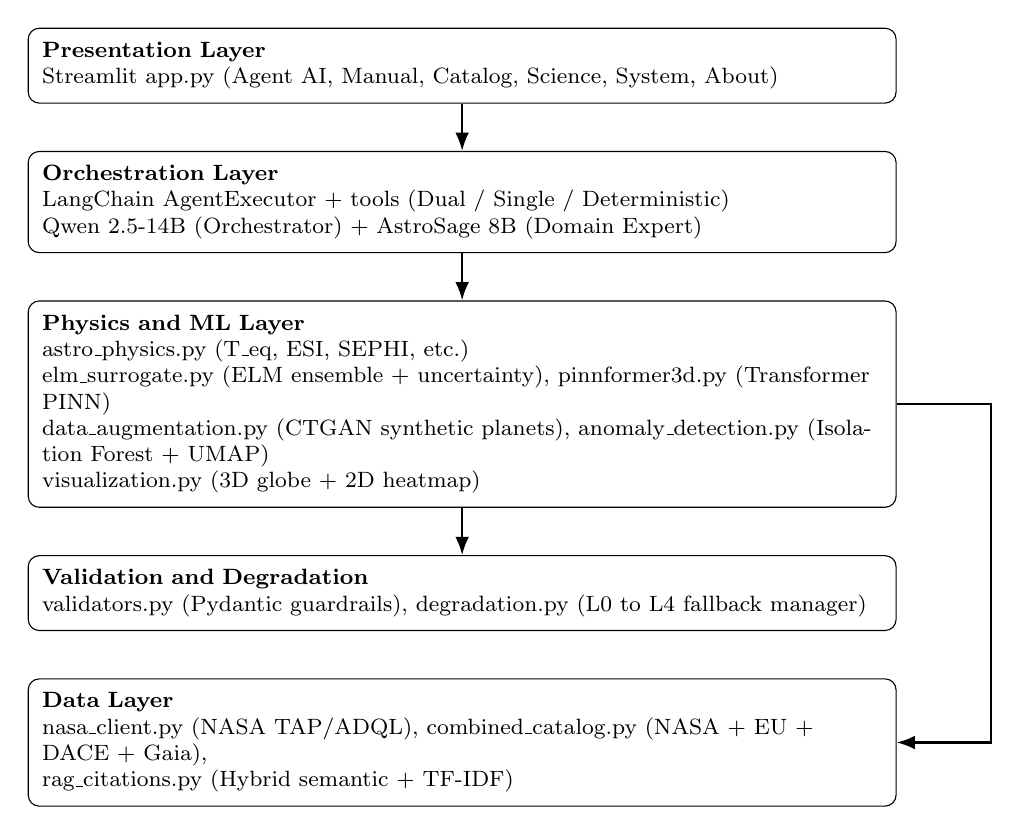
\begin{tikzpicture}[
        node distance=6mm,
        >={Latex[length=2mm]},
        layer/.style={
            rectangle,
            rounded corners,
            draw=black,
            align=left,
            text width=0.88\textwidth,
            inner sep=5pt,
            font=\footnotesize
        },
        arrow/.style={-Latex,thick}
    ]

    \node[layer] (presentation) {
        \textbf{Presentation Layer}\\
        Streamlit app.py (Agent AI, Manual, Catalog, Science, System, About)
    };

    \node[layer, below=of presentation] (orchestration) {
        \textbf{Orchestration Layer}\\
        LangChain AgentExecutor + tools (Dual / Single / Deterministic)\\
        Qwen 2.5-14B (Orchestrator) + AstroSage 8B (Domain Expert)
    };

    \node[layer, below=of orchestration] (physicsml) {
        \textbf{Physics and ML Layer}\\
        astro\_physics.py (T\_eq, ESI, SEPHI, etc.)\\
        elm\_surrogate.py (ELM ensemble + uncertainty), pinnformer3d.py (Transformer PINN)\\
        data\_augmentation.py (CTGAN synthetic planets), anomaly\_detection.py (Isolation Forest + UMAP)\\
        visualization.py (3D globe + 2D heatmap)
    };

    \node[layer, below=of physicsml] (validation) {
        \textbf{Validation and Degradation}\\
        validators.py (Pydantic guardrails), degradation.py (L0 to L4 fallback manager)
    };

    \node[layer, below=of validation] (data) {
        \textbf{Data Layer}\\
        nasa\_client.py (NASA TAP/ADQL), combined\_catalog.py (NASA + EU + DACE + Gaia),\\
        rag\_citations.py (Hybrid semantic + TF-IDF)
    };

    \draw[arrow] (presentation) -- (orchestration);
    \draw[arrow] (orchestration) -- (physicsml);
    \draw[arrow] (physicsml) -- (validation);
    \draw[arrow] (physicsml.east) -- ++(1.2,0) |- (data.east);

    \end{tikzpicture}
    \caption{The high-level architecture of the Autonomous Exoplanetary Digital Twin.}
\end{figure}

\subsection*{Operational data-flow diagrams}

\begin{figure}[H]
    \centering
    \resizebox{\textwidth}{!}{%
    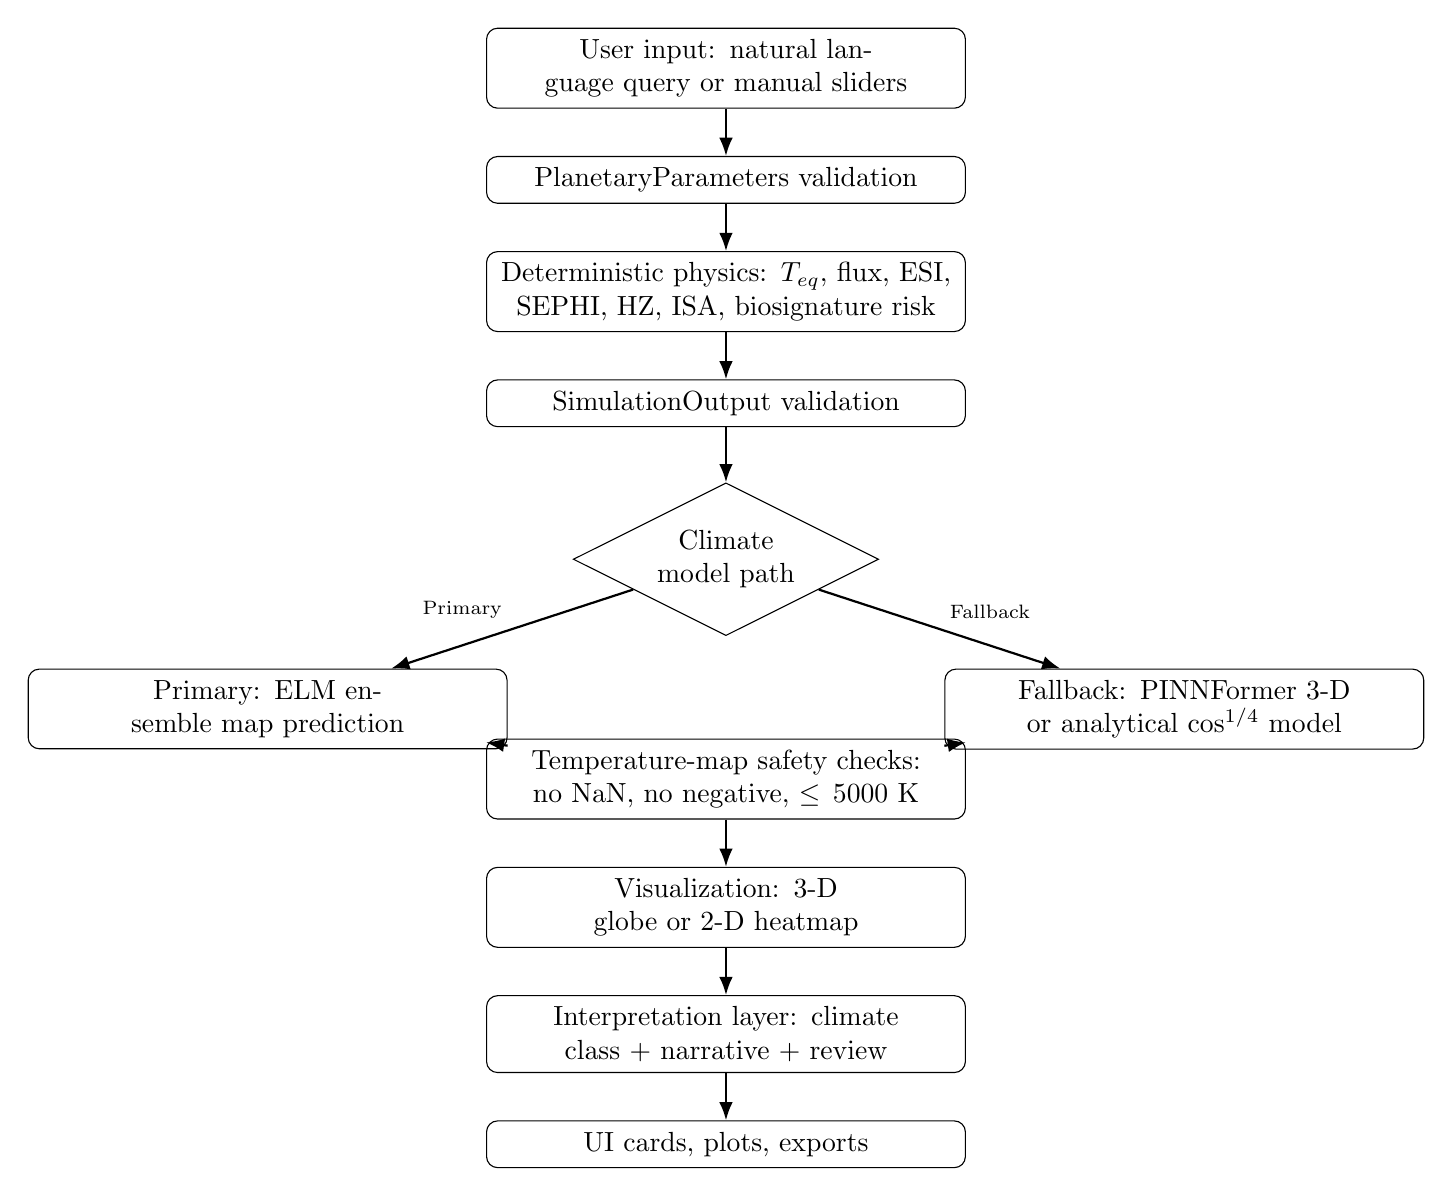
\begin{tikzpicture}[
        node distance=6mm,
        >={Latex[length=2mm]},
        flow/.style={rectangle, rounded corners, draw=black, align=center, inner sep=4pt, text width=5.8cm},
        decision/.style={diamond, draw=black, align=center, aspect=2.0, inner sep=1pt, text width=2.2cm},
        arrow/.style={-Latex, thick}
    ]
    \node[flow] (a) {User input: natural language query or manual sliders};
    \node[flow, below=of a] (b) {PlanetaryParameters validation};
    \node[flow, below=of b] (c) {Deterministic physics: $T_{eq}$, flux, ESI, SEPHI, HZ, ISA, biosignature risk};
    \node[flow, below=of c] (d) {SimulationOutput validation};
    \node[decision, below=7mm of d] (e) {Climate model path};
    \node[flow, below left=9mm and 18mm of e] (f) {Primary: ELM ensemble map prediction};
    \node[flow, below right=9mm and 18mm of e] (g) {Fallback: PINNFormer 3-D or analytical $\cos^{1/4}$ model};
    \node[flow, below=13mm of e] (h) {Temperature-map safety checks: no NaN, no negative, $\leq 5000$ K};
    \node[flow, below=of h] (i) {Visualization: 3-D globe or 2-D heatmap};
    \node[flow, below=of i] (j) {Interpretation layer: climate class + narrative + review};
    \node[flow, below=of j] (k) {UI cards, plots, exports};

    \draw[arrow] (a) -- (b);
    \draw[arrow] (b) -- (c);
    \draw[arrow] (c) -- (d);
    \draw[arrow] (d) -- (e);
    \draw[arrow] (e) -- node[above left, font=\scriptsize] {Primary} (f);
    \draw[arrow] (e) -- node[above right, font=\scriptsize] {Fallback} (g);
    \draw[arrow] (f) -- (h);
    \draw[arrow] (g) -- (h);
    \draw[arrow] (h) -- (i);
    \draw[arrow] (i) -- (j);
    \draw[arrow] (j) -- (k);
    \end{tikzpicture}%
    }
    \caption{End-to-end data flow from user query to simulation output and validated visualization.}
    \label{fig:user_to_simulation_flow}
\end{figure}

\begin{figure}[H]
    \centering
    \resizebox{\textwidth}{!}{%
    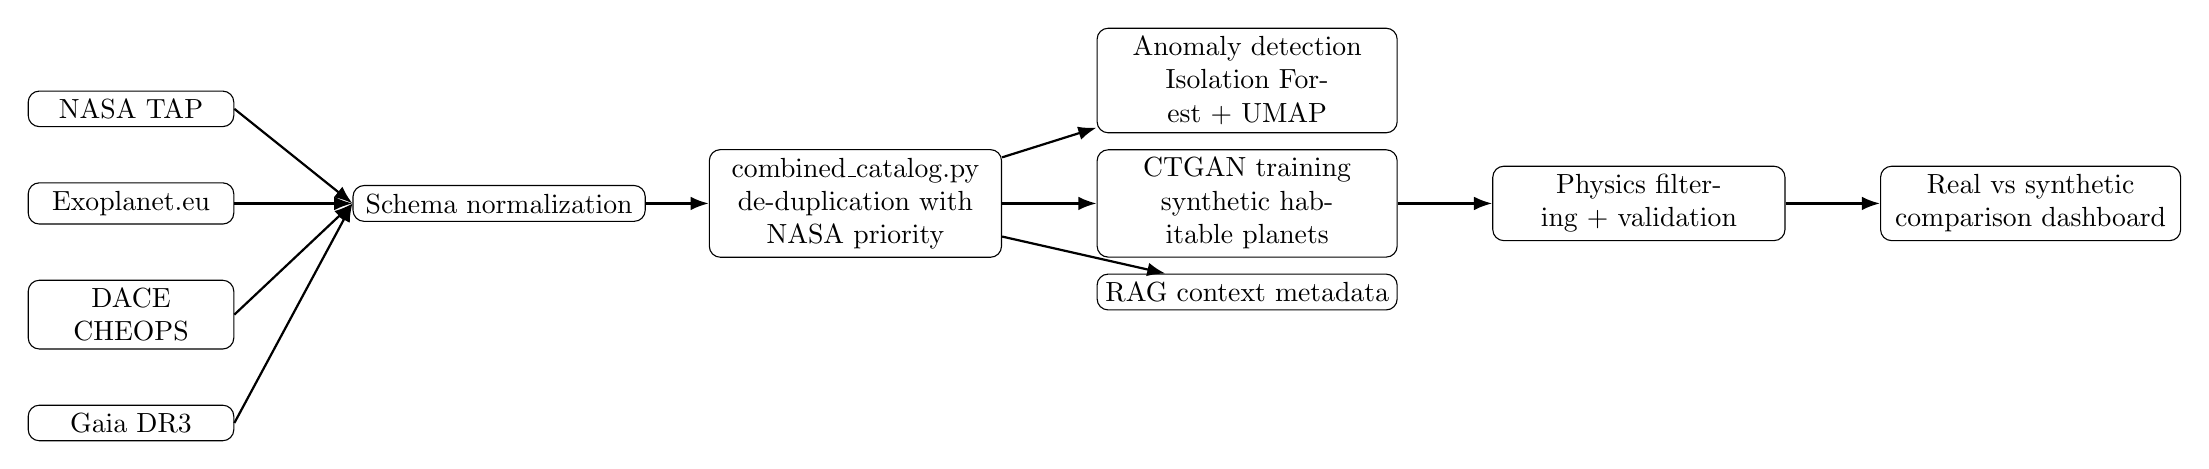
\begin{tikzpicture}[
        node distance=7mm and 8mm,
        >={Latex[length=2mm]},
        src/.style={rectangle, rounded corners, draw=black, align=center, inner sep=3pt, text width=2.4cm},
        proc/.style={rectangle, rounded corners, draw=black, align=center, inner sep=3pt, text width=3.5cm},
        outputbox/.style={rectangle, rounded corners, draw=black, align=center, inner sep=3pt, text width=3.6cm},
        arrow/.style={-Latex, thick}
    ]
    \node[src] (nasa) {NASA TAP};
    \node[src, below=of nasa] (eu) {Exoplanet.eu};
    \node[src, below=of eu] (dace) {DACE CHEOPS};
    \node[src, below=of dace] (gaia) {Gaia DR3};

    \node[proc, right=15mm of eu] (norm) {Schema normalization};
    \node[proc, right=of norm] (comb) {combined\_catalog.py\\de-duplication with NASA priority};

    \node[outputbox, above right=2mm and 12mm of comb] (anom) {Anomaly detection\\Isolation Forest + UMAP};
    \node[outputbox, right=12mm of comb] (ctgan) {CTGAN training\\synthetic habitable planets};
    \node[outputbox, below right=2mm and 12mm of comb] (rag) {RAG context metadata};

    \node[proc, right=12mm of ctgan] (filter) {Physics filtering + validation};
    \node[outputbox, right=12mm of filter] (dash) {Real vs synthetic\\comparison dashboard};

    \draw[arrow] (nasa.east) -- (norm.west);
    \draw[arrow] (eu.east) -- (norm.west);
    \draw[arrow] (dace.east) -- (norm.west);
    \draw[arrow] (gaia.east) -- (norm.west);
    \draw[arrow] (norm) -- (comb);

    \draw[arrow] (comb) -- (anom);
    \draw[arrow] (comb) -- (ctgan);
    \draw[arrow] (comb) -- (rag);
    \draw[arrow] (ctgan) -- (filter);
    \draw[arrow] (filter) -- (dash);
    \end{tikzpicture}%
    }
    \caption{Catalog ingestion and augmentation pipeline from multi-archive sources to anomaly analytics and synthetic-data diagnostics.}
    \label{fig:catalog_ingestion_pipeline}
\end{figure}

\begin{figure}[H]
    \centering
    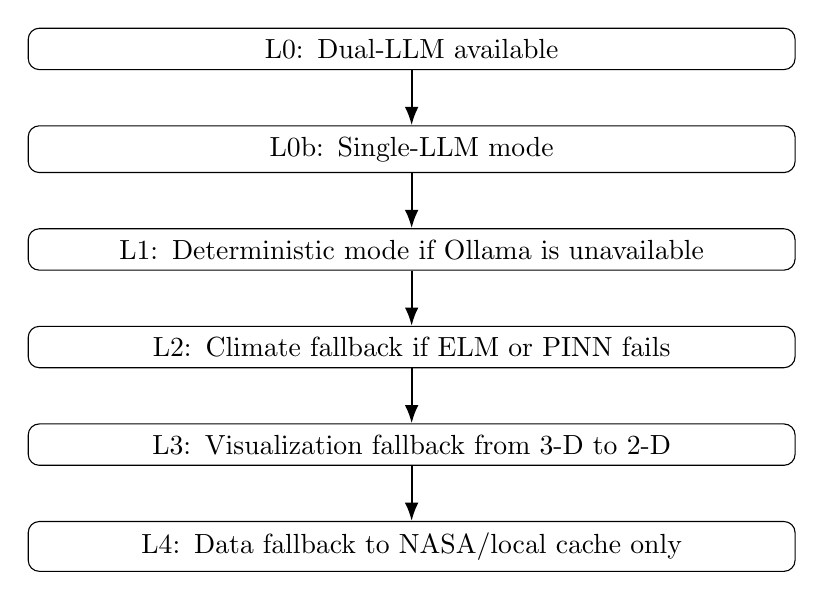
\begin{tikzpicture}[
        node distance=7mm,
        >={Latex[length=2mm]},
        level/.style={rectangle, rounded corners, draw=black, align=center, inner sep=4pt, text width=0.78\textwidth},
        arrow/.style={-Latex, thick}
    ]
    \node[level] (l0) {L0: Dual-LLM available};
    \node[level, below=of l0] (l0b) {L0b: Single-LLM mode};
    \node[level, below=of l0b] (l1) {L1: Deterministic mode if Ollama is unavailable};
    \node[level, below=of l1] (l2) {L2: Climate fallback if ELM or PINN fails};
    \node[level, below=of l2] (l3) {L3: Visualization fallback from 3-D to 2-D};
    \node[level, below=of l3] (l4) {L4: Data fallback to NASA/local cache only};

    \draw[arrow] (l0) -- (l0b);
    \draw[arrow] (l0b) -- (l1);
    \draw[arrow] (l1) -- (l2);
    \draw[arrow] (l2) -- (l3);
    \draw[arrow] (l3) -- (l4);
    \end{tikzpicture}
    \caption{Runtime graceful-degradation cascade used to preserve availability under component failures.}
    \label{fig:degradation_cascade}
\end{figure}
\newpage




% -------------------------------------------------------------------
% 5. IMPLEMENTATION OF THE AI PART
% -------------------------------------------------------------------
\section{Implementation of the AI part}

The AI implementation is not a single model. It is a coordinated set of deterministic and learned modules combined through a validated execution pipeline.

\subsection{Module-level implementation breakdown}

The module-level implementation is organized as a coordinated pipeline in which \path{modules/astro_physics.py} provides deterministic astrophysics calculations
such as equilibrium temperature ($T_{eq}$), stellar flux, Earth-normalized flux, ESI and SEPHI criteria, habitable-zone boundaries, habitable surface fraction, ISA-inspired interaction heuristics, biosignature false-positive risk heuristics,
and composition helpers, while \path{modules/elm_surrogate.py} serves as the default fast climate engine by preparing planetary features, solving the output layer analytically in Moore-Penrose style,
performing ensemble inference for variance reduction, estimating prediction intervals, and loading serialized artifacts like \path{models/elm_ensemble.pkl};
in parallel, \path{modules/pinnformer3d.py} provides an experimental transformer-based physics-informed alternative with configurable presets
(including greenhouse, ocean heat transport, cloud, tidal, ice-albedo, and advection effects) for richer field generation when available, \path{modules/data_augmentation.py} and \path{modules/anomaly_detection.py} 
handle CTGAN-based synthetic data generation with physical post-filtering plus Isolation Forest and UMAP-based anomaly diagnostics, \path{modules/agent_setup.py} and \path{modules/rag_citations.py} provide tool-calling orchestration and citation-grounded retrieval over a curated astrobiology corpus, and \path{modules/validators.py} enforces strict constraints on stellar, planetary, and simulation objects so unphysical values are blocked before they propagate downstream.
\newline


\begin{figure}[H]
    \centering
    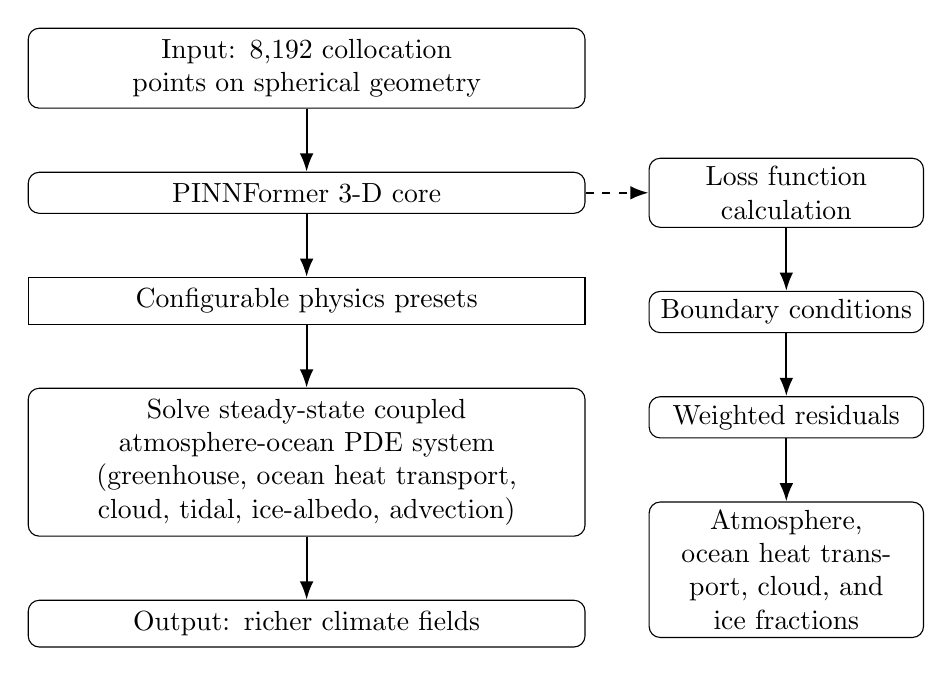
\begin{tikzpicture}[
        node distance=8mm and 10mm,
        >={Latex[length=2mm]},
        box/.style={rectangle, rounded corners, draw=black, align=center, inner sep=4pt, text width=0.56\textwidth},
        decision/.style={rectangle, draw=black, align=center, inner sep=4pt, text width=0.56\textwidth},
        side/.style={rectangle, rounded corners, draw=black, align=center, inner sep=3pt, text width=0.27\textwidth},
        arrow/.style={-Latex, thick},
        dashedarrow/.style={-Latex, thick, dashed}
    ]

    \node[box] (a) {Input: 8,192 collocation points on spherical geometry};
    \node[box, below=of a] (b) {PINNFormer 3-D core};
    \node[decision, below=of b] (c) {Configurable physics presets};
    \node[box, below=of c] (d) {Solve steady-state coupled atmosphere-ocean PDE system\\(greenhouse, ocean heat transport, cloud, tidal, ice-albedo, advection)};
    \node[box, below=of d] (e) {Output: richer climate fields};

    \node[side, right=8mm of b] (f) {Loss function calculation};
    \node[side, below=of f] (g) {Boundary conditions};
    \node[side, below=of g] (h) {Weighted residuals};
    \node[side, below=of h] (i) {Atmosphere, ocean heat transport, cloud, and ice fractions};

    \draw[arrow] (a) -- (b);
    \draw[arrow] (b) -- (c);
    \draw[arrow] (c) -- (d);
    \draw[arrow] (d) -- (e);

    \draw[dashedarrow] (b.east) -- (f.west);
    \draw[arrow] (f) -- (g);
    \draw[arrow] (g) -- (h);
    \draw[arrow] (h) -- (i);

    \end{tikzpicture}
    \caption{PINNFormer 3-D execution flow and physics-constrained loss structure}
    \label{fig:pinnformer_flow}
\end{figure}






\subsection{Core AI implemenation details}


For climate map generation, we use an Extreme Learning Machine (ELM) ensemble, a single-hidden-layer feedforward neural network where input weights are frozen and output weights are solved analytically via the Moore-Penrose pseudoinverse:
\begin{equation}
\beta = \left(H^T H + \frac{I}{C}\right)^{-1} H^T T
\label{eq:elm_output_weights}
\end{equation}
where $\beta$ is the output-weight matrix, $H$ is the hidden-layer activation matrix, $H^T$ denotes the transpose of $H$, $I$ is the identity matrix, $C$ is the regularization coefficient, and $T$ is the target output matrix; we use an ensemble of $K=10$ independent ELM models (500 hidden neurons each) to predict a flattened $32 \times 64$ dimensional temperature map from 8 planetary input features, and to address class imbalance we train a Conditional Tabular GAN (CTGAN) with log1p transforms on heavy-tailed features and conditioning on a binary habitable label to generate large sets of physically valid synthetic planets for ELM training; we also include an experimental Transformer-based Physics-Informed Neural Network (PINNFormer 3-D) that uses 8,192 collocation points on spherical geometry to solve a steady-state coupled atmosphere-ocean PDE system with boundary-condition and weighted-residual losses for atmosphere, ocean heat transport, cloud, and ice fractions; for scientific grounding we use a hybrid Retrieval-Augmented Generation pipeline with ChromaDB over 40 peer-reviewed astrobiology papers, combining sentence-transformer semantic retrieval with TF-IDF keyword retrieval through Reciprocal Rank Fusion; for catalog diagnostics we apply Isolation Forest-based anomaly detection with UMAP 2D projection to analyze outliers and structure in both real and synthetic samples; and for reliability we combine runtime validators with targeted automated tests and dedicated diagnostics that benchmark ELM predictions against synthetic GCM reference profiles and compare CTGAN-generated distributions with real catalog data.
\newpage




% -------------------------------------------------------------------
% 6. SIMULATION RESULTS FROM THE APPLICATION
% -------------------------------------------------------------------
\section{Simulation results from the application}

This section reports observed outcomes across four representative scenarios and summarizes their habitability implications.

\begin{table}[H]
    \centering
    \begin{tabularx}{\textwidth}{l l c c c X}
        \toprule
        \textbf{Key input profile} & \textbf{$T_{eq}$ [K]} & \textbf{ESI} & \textbf{SEPHI} & \textbf{HSF} & \textbf{Interpretation} \\
        \midrule
        Earth-like & 255 K & 0.916 & 0.67 & 91.9\% & Earth-like conditions \\
        Tidally locked & 272 K & 0.944 & 0.67 & 37.0\% & Potentially habitable \\
        Hot rocky control & 1449 K & 0.203 & 0.67 & 0.0\% & Uninhabitable \\
        Catalog anomalies & 167.34 K & 0.2957 & 0.33 & 15.44\% & Uninhabitable \\
        \bottomrule
    \end{tabularx}
\end{table}


The simulation results from our application demonstrate massive computational speedups.
The ELM Ensemble generates a full $32 \times 64$ climate surface-temperature map in $<100$ milliseconds on a standard CPU,
effectively bypassing the multi-day bottleneck of GCMs. 
Overall, the scenario suite demonstrates that the system distinguishes plausibly habitable, marginal, and non-habitable regimes while preserving rapid inference and interpretable diagnostics.
\newline



\textbf{Second Scenario: Tidally locked habitable candidate}
\newline
A tidally locked candidate yielded $T_{eq}=272$ K, ESI $=0.944$, SEPHI $=0.67$, and HSF $=37.0\%$. The cross-section profile shows a strong day-night gradient with a temperate transition zone, consistent with an eyeball-like climate pattern.


\begin{figure}[H]
    \centering
    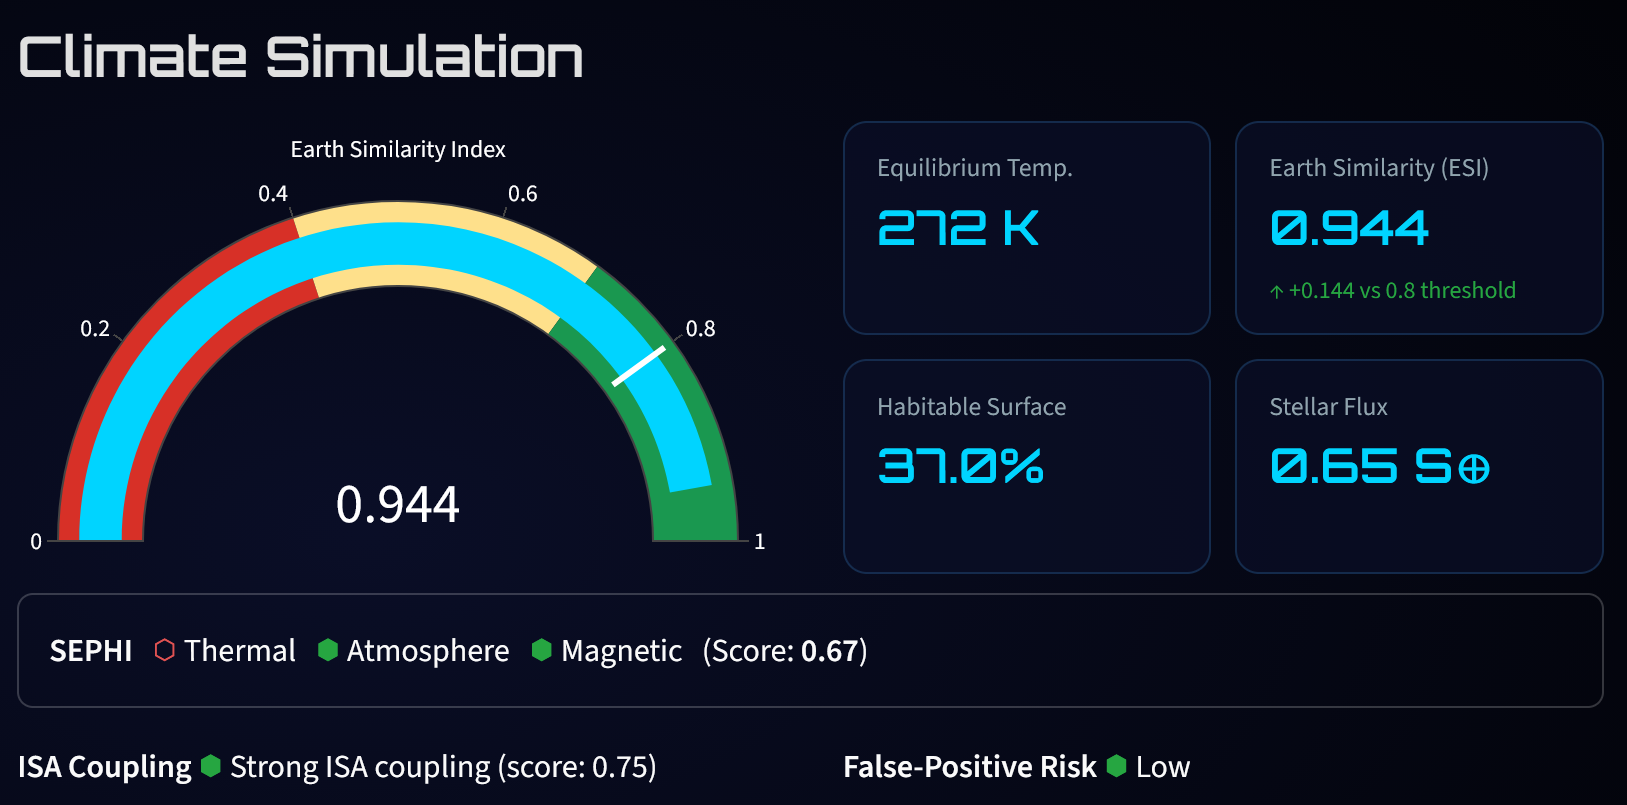
\includegraphics[width=0.7\textwidth]{app-photos/ESI.png}
    \caption{Climate simulation dashboard showing key diagnostics, including equilibrium temperature, Earth Similarity Index (ESI), SEPHI components, and habitable surface fraction.}
    \label{fig:esi_dashboard}
\end{figure}


\begin{figure}[H]
    \centering
    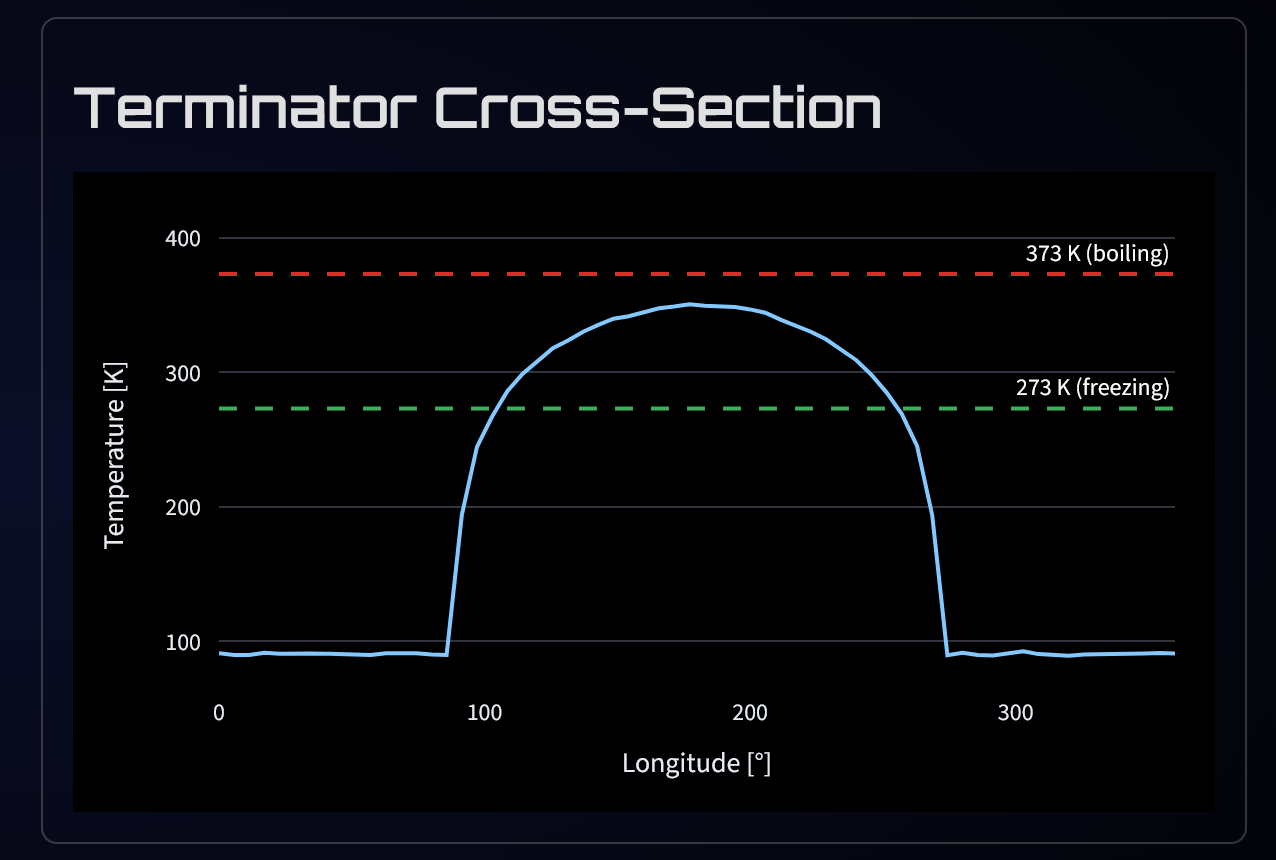
\includegraphics[width=0.5\textwidth]{app-photos/cross-section.png}
    \caption{Terminator cross-section temperature profile for a tidally locked candidate, highlighting the day-night thermal gradient and the temperate transition zone.}
    \label{fig:terminator_cross_section}
\end{figure}


\begin{figure}[H]
    \centering
    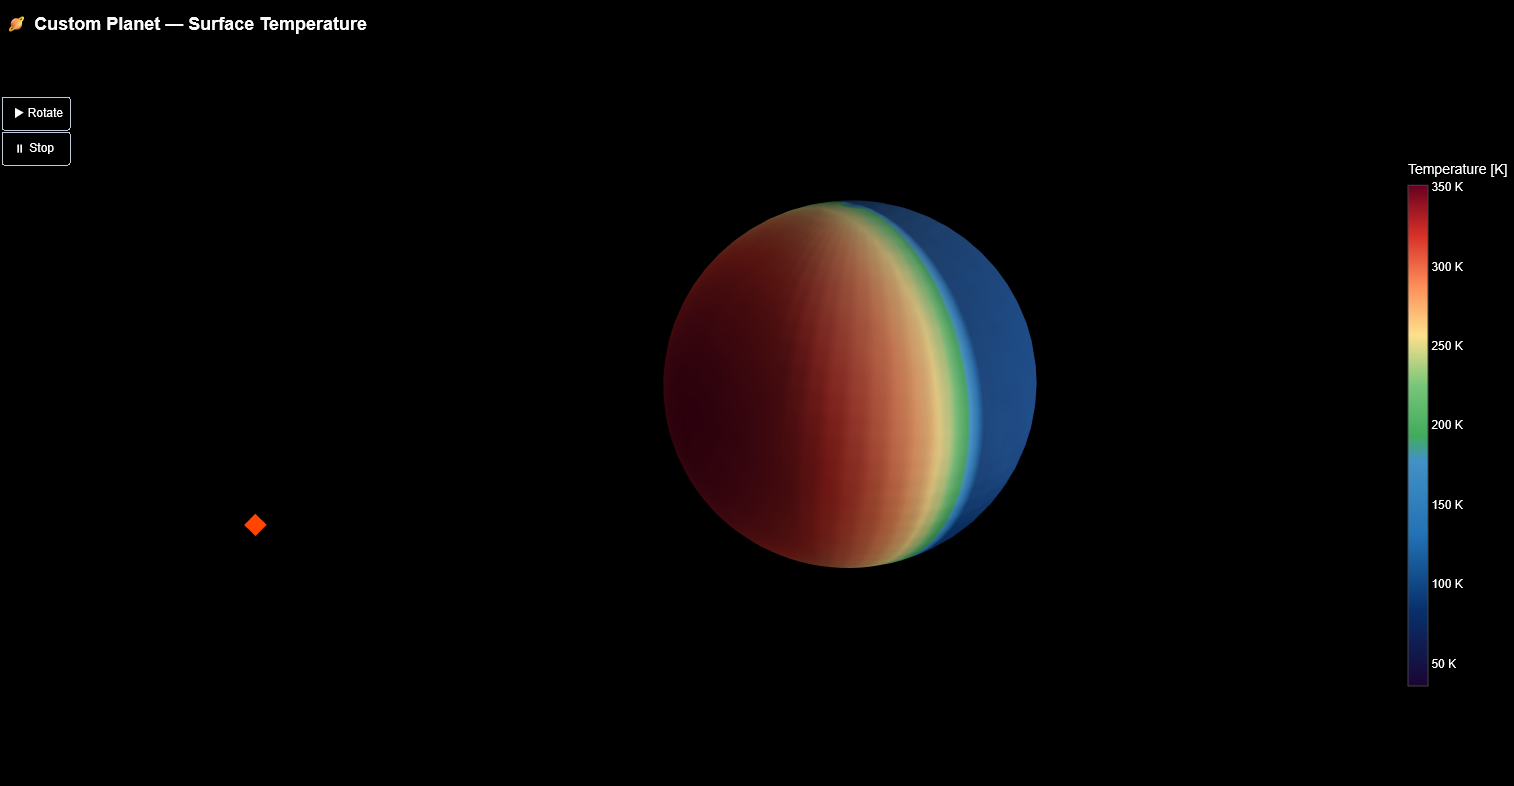
\includegraphics[width=0.8\textwidth]{app-photos/globe.png}
    \caption{3D interactive globe of predicted surface temperature mapped in Plotly.}
\end{figure}

When rendering tidally locked planets (like Proxima Centauri b), the model correctly produces an "Eyeball" climate state-showing a hot substellar point surrounded by global ice. The CTGAN successfully generated 500,000 synthetic planetary data points, and our physical post-filter ensured that outputs stayed strictly within thermodynamic bounds (e.g., $T_{eq} \in [10, 4000]$ K). 

\begin{figure}[H]
    \centering
    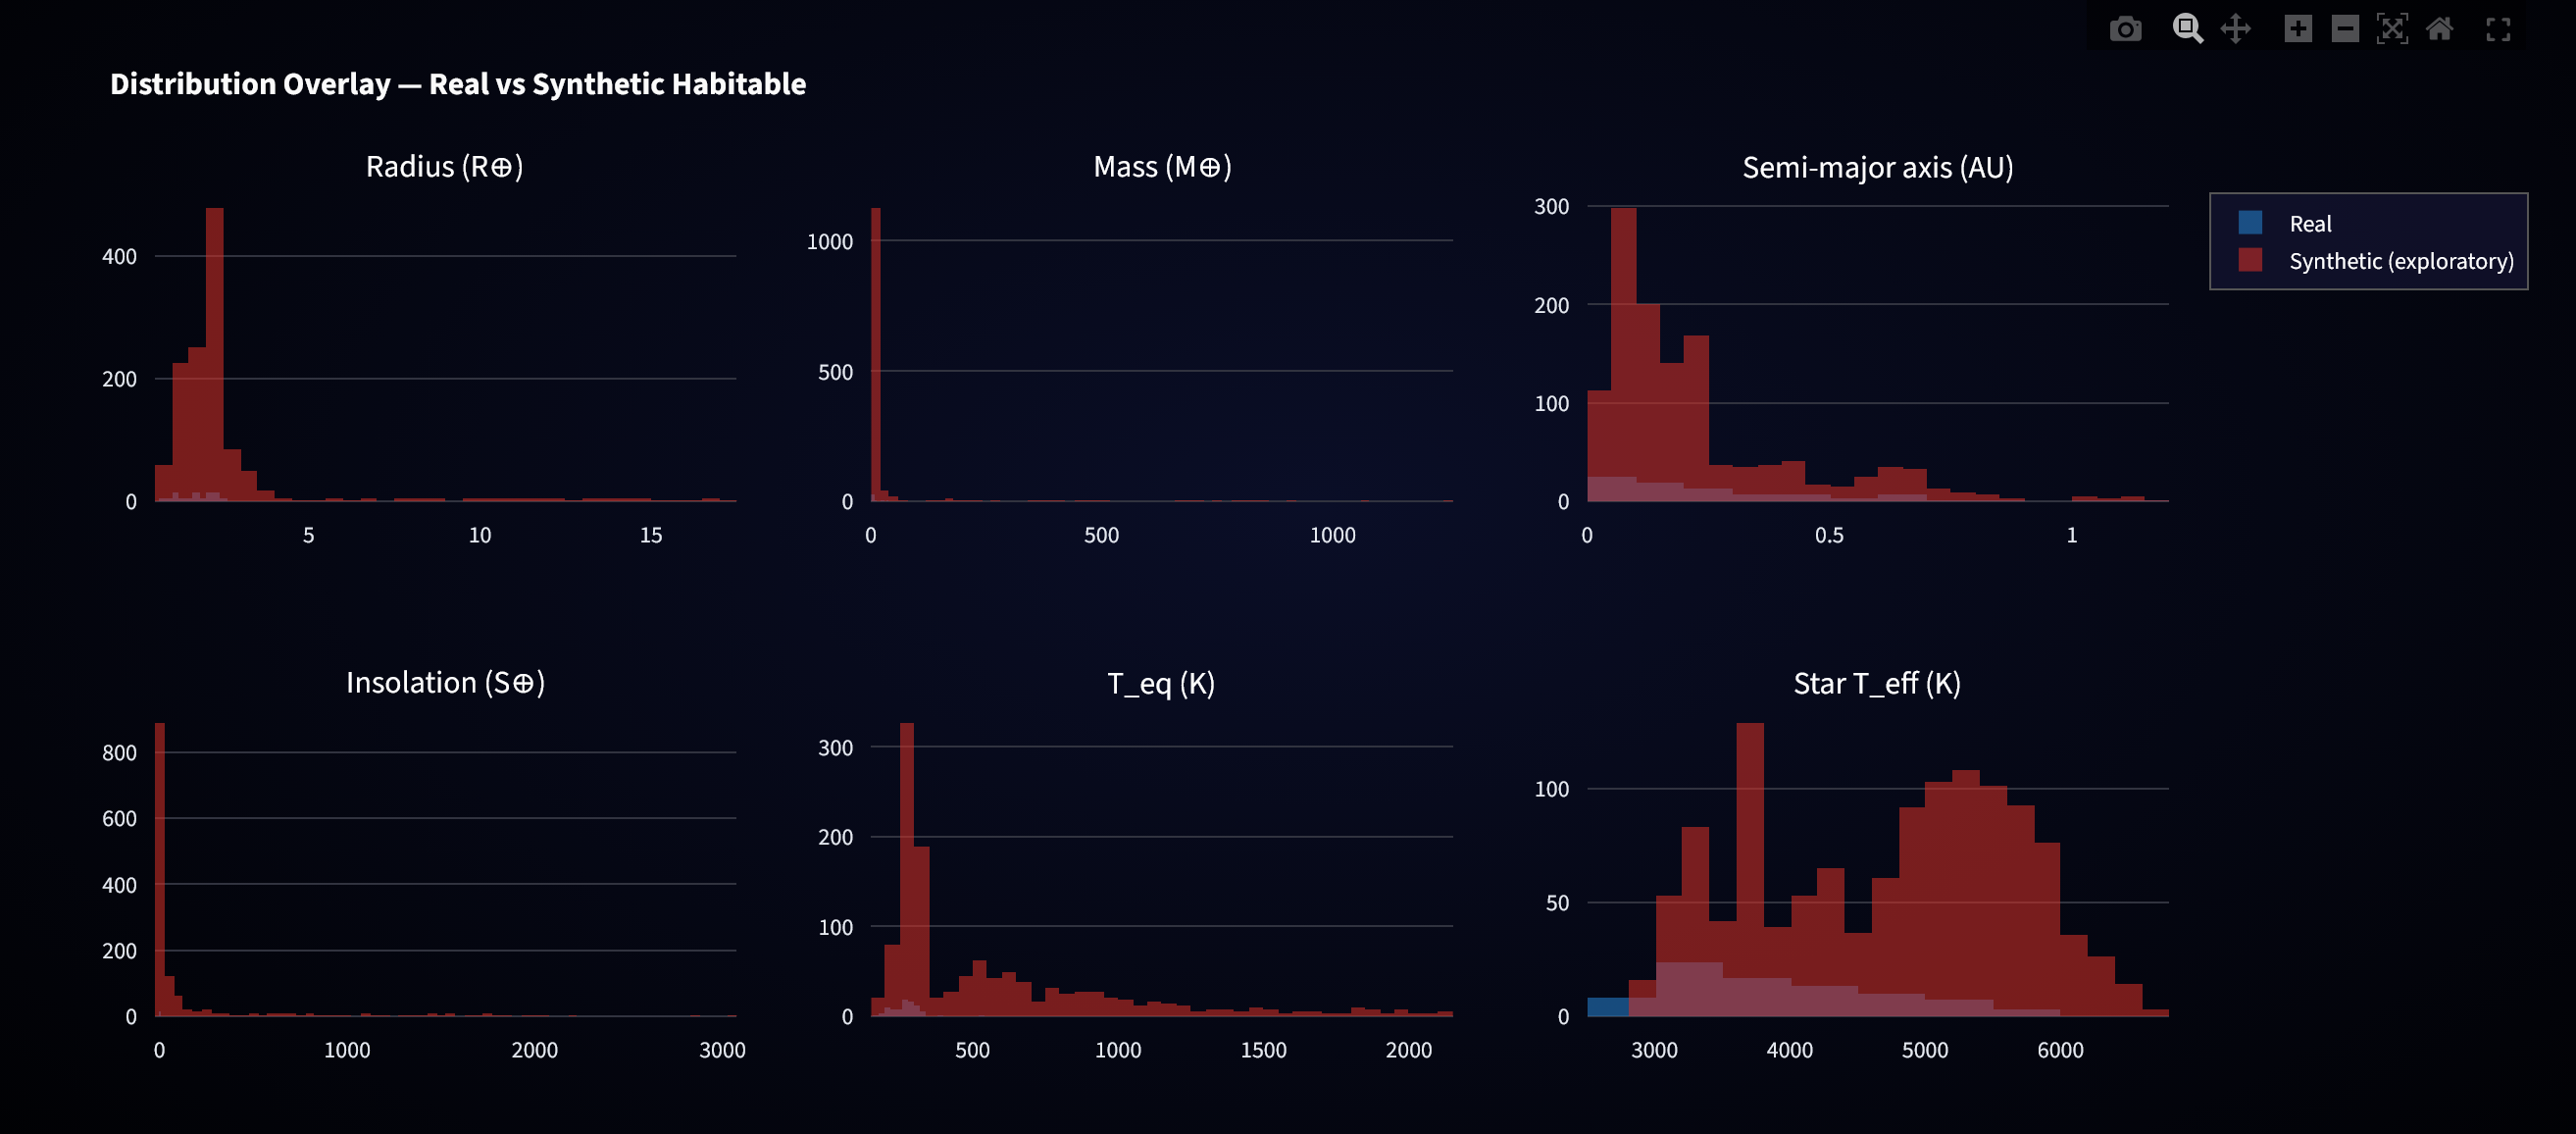
\includegraphics[width=\textwidth]{app-photos/Zrzut ekranu 2026-03-18 143705.png}
    \caption{Distribution overlay comparing real catalog planets and synthetic habitable candidates generated by CTGAN across key physical parameters.}
    \label{fig:ctgan_distribution_overlay}
\end{figure}

Comparisons against precomputed GCM benchmark profiles (e.g., Earth-like aquaplanets and hot rocks) show strong pattern correlation, proving the ELM acts as a viable hypothesis-generating approximation. Furthermore, the Isolation Forest anomaly detection successfully clustered the NASA catalog, identifying outliers and displaying them effectively using UMAP 2D projections.

\begin{figure}[H]
    \centering
    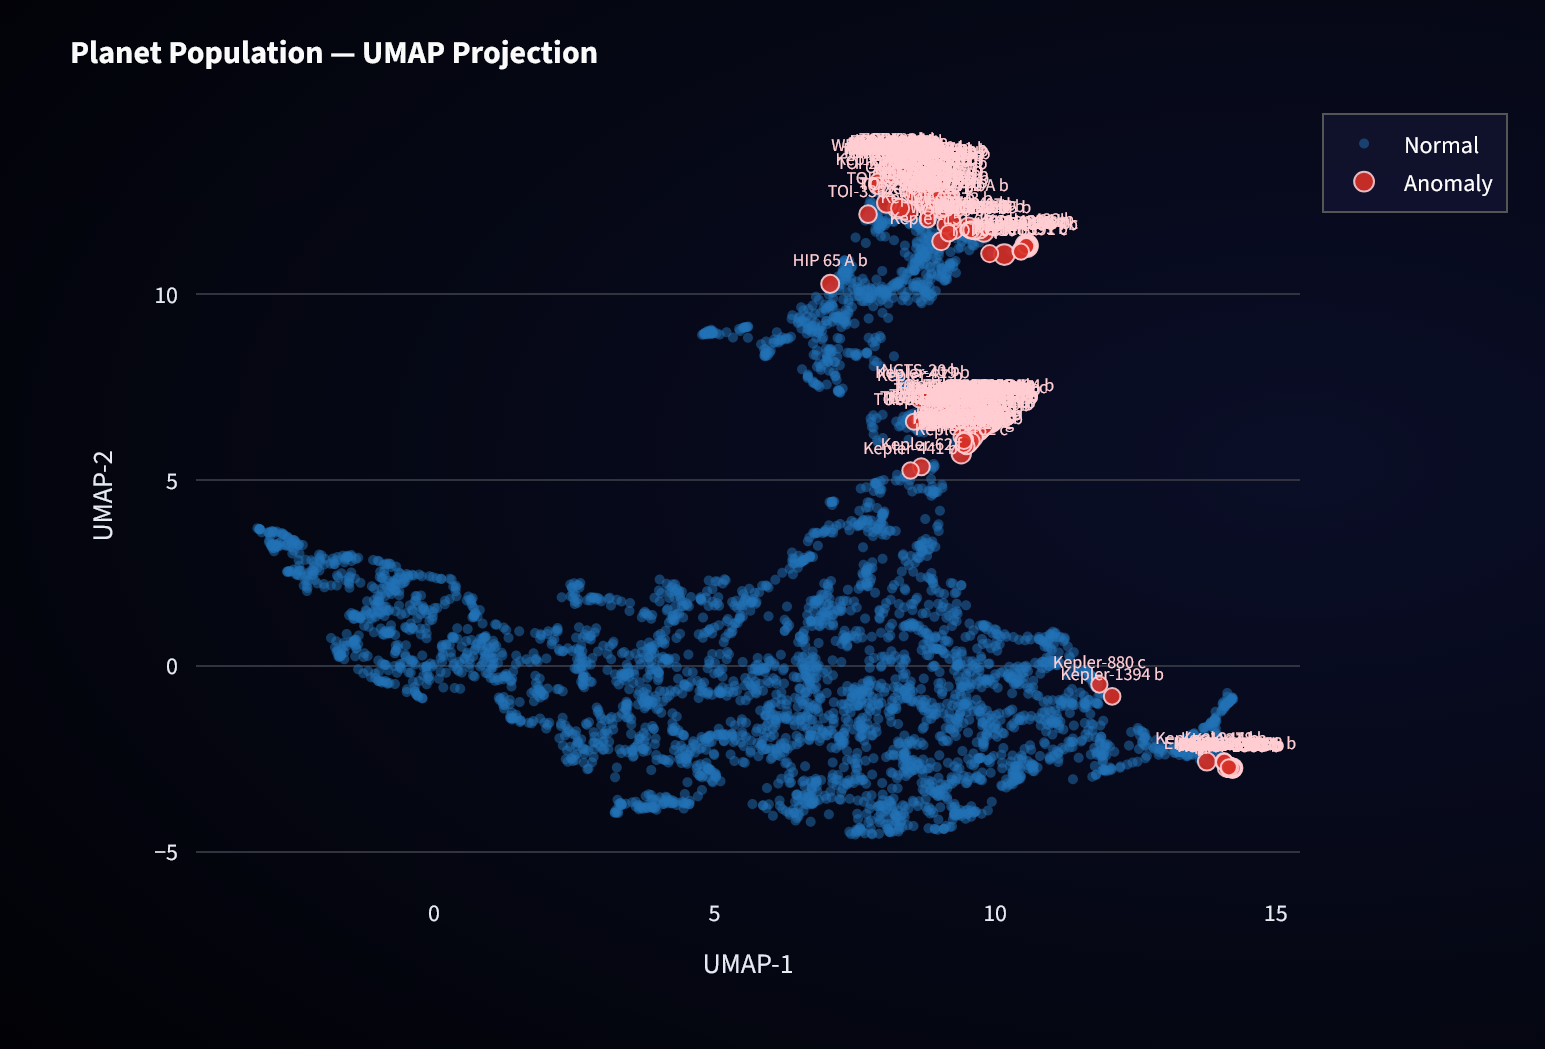
\includegraphics[width=0.9\textwidth]{app-photos/umap.png}
    \caption{UMAP 2D projection of catalog planets, with anomaly candidates highlighted by the Isolation Forest-based detection module.}
    \label{fig:umap_projection}
\end{figure}



\newpage

% -------------------------------------------------------------------
% 7. CONCLUSIONS
% -------------------------------------------------------------------
\section{Conclusions}

The Autonomous Exoplanetary Digital Twin successfully demonstrates that fast, data-driven ML models combined with physics guardrails can serve as effective climate surrogates. The app has very good results with generating instantaneous climate approximations and assessing habitability metrics. 

However, as addressed in our critique response, there are known limitations. The ELM ensemble is currently trained on analytically generated data rather than being calibrated directly against full ROCKE-3D outputs, meaning the surrogate currently models simplified radiative-equilibrium physics. Photosynthesis limits, realistic atmospheric escape modeling, and dynamically computed albedos (rather than static slider inputs) represent areas for improvement.

Future work will focus on integrating a lightweight GCM (like ExoPlaSim) directly into the fallback cascade and utilizing real GCM temperature maps to train the next iteration of the ELM surrogate.


% -------------------------------------------------------------------
% LITERATURE
% -------------------------------------------------------------------
\section*{Literature}
\begin{enumerate}
    \item \textbf{Huang, G.-B., Zhu, Q.-Y., Siew, C.-K.}: \textit{Extreme Learning Machine: Theory and Applications}. Neurocomputing, 70(1-3), 489–501 (2006).
    \item \textbf{Kopparapu, R. K., et al.}: \textit{Habitable Zones around Main-Sequence Stars}. The Astrophysical Journal, 765(2), 131 (2013).
    \item \textbf{Schulze-Makuch, D., et al.}: \textit{A Two-Tiered Approach to Assessing the Habitability of Exoplanets}. Astrobiology, 11(10), 1041–1052 (2011).
    \item \textbf{Chen, J., Kipping, D.}: \textit{Probabilistic Forecasting of the Masses and Radii of Other Worlds}. The Astrophysical Journal, 834(1), 17 (2017).
    \item \textbf{Rodríguez-Mozos, J. M., Moya, A.}: \textit{Statistical-Likelihood Exo-Planetary Habitability Index (SEPHI)}. MNRAS, 471(4), 4628–4636 (2017).
\end{enumerate}

\end{document}

